
\documentclass[border=1pt, crop, multi, tikz]{standalone} 
\usepackage{import}
\subimport{/home/thesis/PlotNeuralNets/layers/}{init}
\usetikzlibrary{positioning}
\usetikzlibrary{3d} %for including external image 

\def\ConvColor{rgb:yellow,5;red,2.5;white,5}
\def\ConvReluColor{rgb:yellow,5;red,5;white,5}
\def\PoolColor{rgb:red,1;black,0.3}
\def\UnpoolColor{rgb:blue,2;green,1;black,0.3}
\def\FcColor{rgb:blue,5;red,2.5;white,5}
\def\FcReluColor{rgb:blue,5;red,5;white,4}
\def\SoftmaxColor{rgb:magenta,5;black,7}   
\def\SumColor{rgb:blue,5;green,15}

\newcommand{\copymidarrow}{\tikz \draw[-Stealth,line width=0.8mm,draw={rgb:blue,4;red,1;green,1;black,3}] (-0.3,0) -- ++(0.3,0);}

\begin{document}
\begin{tikzpicture}
\tikzstyle{connection}=[ultra thick,every node/.style={sloped,allow upside down},draw=\edgecolor,opacity=0.7]
\tikzstyle{copyconnection}=[ultra thick,every node/.style={sloped,allow upside down},draw={rgb:blue,4;red,1;green,1;black,3},opacity=0.7]

\node[canvas is zy plane at x=0] (temp) at (-3,0,0) {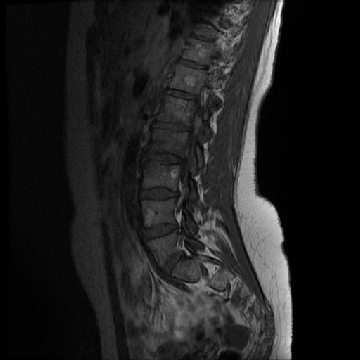
\includegraphics[width=8cm,height=8cm]{/home/thesis/PlotNeuralNets/images/input.png}};

\pic[shift={ (0,0,0) }] at (0,0,0) 
    {RightBandedBox={
        name=ccr_b1,
        caption= ,
        xlabel={{ 64,64 }},
        zlabel=500,
        fill=\ConvColor,
        bandfill=\ConvReluColor,
        height=40,
        width={ 2,2 },
        depth=40
        }
    };

\pic[shift={ (0,0,0) }] at (ccr_b1-east) 
    {Box={
        name=pool_b1,
        caption= ,
        fill=\PoolColor,
        opacity=0.5,
        height=32,
        width=1,
        depth=32
        }
    };

\pic[shift={ (1,0,0) }] at (pool_b1-east) 
    {RightBandedBox={
        name=ccr_b2,
        caption= ,
        xlabel={{ 128,128 }},
        zlabel=256,
        fill=\ConvColor,
        bandfill=\ConvReluColor,
        height=32,
        width={ 3.5,3.5 },
        depth=32
        }
    };

\pic[shift={ (0,0,0) }] at (ccr_b2-east) 
    {Box={
        name=pool_b2,
        caption= ,
        fill=\PoolColor,
        opacity=0.5,
        height=24,
        width=1,
        depth=24
        }
    };

\draw [connection]  (pool_b1-east)    -- node {\midarrow} (ccr_b2-west); % end to_connection

\pic[shift={ (1,0,0) }] at (pool_b2-east) 
    {RightBandedBox={
        name=ccr_b3,
        caption= ,
        xlabel={{ 256,256 }},
        zlabel=128,
        fill=\ConvColor,
        bandfill=\ConvReluColor,
        height=25,
        width={ 4.5,4.5 },
        depth=25
        }
    };

\pic[shift={ (0,0,0) }] at (ccr_b3-east) 
    {Box={
        name=pool_b3,
        caption= ,
        fill=\PoolColor,
        opacity=0.5,
        height=19,
        width=1,
        depth=19
        }
    };

\draw [connection]  (pool_b2-east)    -- node {\midarrow} (ccr_b3-west); % end to_connection

\pic[shift={ (1,0,0) }] at (pool_b3-east) 
    {RightBandedBox={
        name=ccr_b4,
        caption= ,
        xlabel={{ 512,512 }},
        zlabel=64,
        fill=\ConvColor,
        bandfill=\ConvReluColor,
        height=16,
        width={ 5.5,5.5 },
        depth=16
        }
    };

\pic[shift={ (0,0,0) }] at (ccr_b4-east) 
    {Box={
        name=pool_b4,
        caption= ,
        fill=\PoolColor,
        opacity=0.5,
        height=12,
        width=1,
        depth=12
        }
    };

\draw [connection]  (pool_b3-east)    -- node {\midarrow} (ccr_b4-west); % end to_connection

\pic[shift={ (2,0,0) }] at (pool_b4-east) 
    {RightBandedBox={
        name=ccr_b5,
        caption=Bottleneck,
        xlabel={{ 1024,1024 }},
        zlabel=32,
        fill=\ConvColor,
        bandfill=\ConvReluColor,
        height=8,
        width={ 8,8 },
        depth=8
        }
    };

\draw [connection]  (pool_b4-east)    -- node {\midarrow} (ccr_b5-west); % end to_connection
% to_UnPool
\pic[shift={ (2.1,0,0) }] at (ccr_b5-east) 
    {Box={
        name=unpool_b6,
        caption= ,
        fill=\UnpoolColor,
        opacity=0.5,
        height=16,
        width=1,
        depth=16
        }
    };
% to_ConvRes 1
\pic[shift={ (0,0,0) }] at (unpool_b6-east) 
    {RightBandedBox={
        name=ccr_res_b6,
        caption= ,
        xlabel={{ 512, }},
        zlabel=64,
        fill={rgb:white,1;black,3},
        bandfill={rgb:white,1;black,2},
        opacity=0.5,
        height=16,
        width=5.0,
        depth=16
        }
    };
%to_Conv 1
\pic[shift={(0,0,0)}] at (ccr_res_b6-east) 
    {Box={
        name=ccr_b6,
        caption= ,
        xlabel={{512, }},
        zlabel=64,
        fill=\ConvColor,
        height=16,
        width=5.0,
        depth=16
        }
    };
% to_ConvRes 2
\pic[shift={ (0,0,0) }] at (ccr_b6-east) 
    {RightBandedBox={
        name=ccr_res_c_b6,
        caption= ,
        xlabel={{ 512, }},
        zlabel=64,
        fill={rgb:white,1;black,3},
        bandfill={rgb:white,1;black,2},
        opacity=0.5,
        height=16,
        width=5.0,
        depth=16
        }
    };
% to_Conv 2
\pic[shift={(0,0,0)}] at (ccr_res_c_b6-east) 
    {Box={
        name=end_b6,
        caption= ,
        xlabel={{512, }},
        zlabel=64,
        fill=\ConvColor,
        height=16,
        width=5.0,
        depth=16
        }
    };
% to_connection
\draw [connection]  (ccr_b5-east)    -- node {\midarrow} (unpool_b6-west); % end to_connection

\path (ccr_b4-southeast) -- (ccr_b4-northeast) coordinate[pos=1.25] (ccr_b4-top) ;
\path (ccr_res_b6-south)  -- (ccr_res_b6-north)  coordinate[pos=1.25] (ccr_res_b6-top) ;
\draw [copyconnection]  (ccr_b4-northeast)  
-- node {\copymidarrow}(ccr_b4-top)
-- node {\copymidarrow}(ccr_res_b6-top)
-- node {\copymidarrow} (ccr_res_b6-north);
% to_UnPool
\pic[shift={ (2.1,0,0) }] at (end_b6-east) 
    {Box={
        name=unpool_b7,
        caption= ,
        fill=\UnpoolColor,
        opacity=0.5,
        height=25,
        width=1,
        depth=25
        }
    };
% to_ConvRes 1
\pic[shift={ (0,0,0) }] at (unpool_b7-east) 
    {RightBandedBox={
        name=ccr_res_b7,
        caption= ,
        xlabel={{ 256, }},
        zlabel=128,
        fill={rgb:white,1;black,3},
        bandfill={rgb:white,1;black,2},
        opacity=0.5,
        height=25,
        width=4.5,
        depth=25
        }
    };
%to_Conv 1
\pic[shift={(0,0,0)}] at (ccr_res_b7-east) 
    {Box={
        name=ccr_b7,
        caption= ,
        xlabel={{256, }},
        zlabel=128,
        fill=\ConvColor,
        height=25,
        width=4.5,
        depth=25
        }
    };
% to_ConvRes 2
\pic[shift={ (0,0,0) }] at (ccr_b7-east) 
    {RightBandedBox={
        name=ccr_res_c_b7,
        caption= ,
        xlabel={{ 256, }},
        zlabel=128,
        fill={rgb:white,1;black,3},
        bandfill={rgb:white,1;black,2},
        opacity=0.5,
        height=25,
        width=4.5,
        depth=25
        }
    };
% to_Conv 2
\pic[shift={(0,0,0)}] at (ccr_res_c_b7-east) 
    {Box={
        name=end_b7,
        caption= ,
        xlabel={{256, }},
        zlabel=128,
        fill=\ConvColor,
        height=25,
        width=4.5,
        depth=25
        }
    };
% to_connection
\draw [connection]  (end_b6-east)    -- node {\midarrow} (unpool_b7-west); % end to_connection

\path (ccr_b3-southeast) -- (ccr_b3-northeast) coordinate[pos=1.25] (ccr_b3-top) ;
\path (ccr_res_b7-south)  -- (ccr_res_b7-north)  coordinate[pos=1.25] (ccr_res_b7-top) ;
\draw [copyconnection]  (ccr_b3-northeast)  
-- node {\copymidarrow}(ccr_b3-top)
-- node {\copymidarrow}(ccr_res_b7-top)
-- node {\copymidarrow} (ccr_res_b7-north);
% to_UnPool
\pic[shift={ (2.1,0,0) }] at (end_b7-east) 
    {Box={
        name=unpool_b8,
        caption= ,
        fill=\UnpoolColor,
        opacity=0.5,
        height=32,
        width=1,
        depth=32
        }
    };
% to_ConvRes 1
\pic[shift={ (0,0,0) }] at (unpool_b8-east) 
    {RightBandedBox={
        name=ccr_res_b8,
        caption= ,
        xlabel={{ 128, }},
        zlabel=128,
        fill={rgb:white,1;black,3},
        bandfill={rgb:white,1;black,2},
        opacity=0.5,
        height=32,
        width=3.5,
        depth=32
        }
    };
%to_Conv 1
\pic[shift={(0,0,0)}] at (ccr_res_b8-east) 
    {Box={
        name=ccr_b8,
        caption= ,
        xlabel={{128, }},
        zlabel=128,
        fill=\ConvColor,
        height=32,
        width=3.5,
        depth=32
        }
    };
% to_ConvRes 2
\pic[shift={ (0,0,0) }] at (ccr_b8-east) 
    {RightBandedBox={
        name=ccr_res_c_b8,
        caption= ,
        xlabel={{ 128, }},
        zlabel=128,
        fill={rgb:white,1;black,3},
        bandfill={rgb:white,1;black,2},
        opacity=0.5,
        height=32,
        width=3.5,
        depth=32
        }
    };
% to_Conv 2
\pic[shift={(0,0,0)}] at (ccr_res_c_b8-east) 
    {Box={
        name=end_b8,
        caption= ,
        xlabel={{128, }},
        zlabel=128,
        fill=\ConvColor,
        height=32,
        width=3.5,
        depth=32
        }
    };
% to_connection
\draw [connection]  (end_b7-east)    -- node {\midarrow} (unpool_b8-west); % end to_connection

\path (ccr_b2-southeast) -- (ccr_b2-northeast) coordinate[pos=1.25] (ccr_b2-top) ;
\path (ccr_res_b8-south)  -- (ccr_res_b8-north)  coordinate[pos=1.25] (ccr_res_b8-top) ;
\draw [copyconnection]  (ccr_b2-northeast)  
-- node {\copymidarrow}(ccr_b2-top)
-- node {\copymidarrow}(ccr_res_b8-top)
-- node {\copymidarrow} (ccr_res_b8-north);
% to_UnPool
\pic[shift={ (2.1,0,0) }] at (end_b8-east) 
    {Box={
        name=unpool_b9,
        caption= ,
        fill=\UnpoolColor,
        opacity=0.5,
        height=40,
        width=1,
        depth=40
        }
    };
% to_ConvRes 1
\pic[shift={ (0,0,0) }] at (unpool_b9-east) 
    {RightBandedBox={
        name=ccr_res_b9,
        caption= ,
        xlabel={{ 64, }},
        zlabel=512,
        fill={rgb:white,1;black,3},
        bandfill={rgb:white,1;black,2},
        opacity=0.5,
        height=40,
        width=2.5,
        depth=40
        }
    };
%to_Conv 1
\pic[shift={(0,0,0)}] at (ccr_res_b9-east) 
    {Box={
        name=ccr_b9,
        caption= ,
        xlabel={{64, }},
        zlabel=512,
        fill=\ConvColor,
        height=40,
        width=2.5,
        depth=40
        }
    };
% to_ConvRes 2
\pic[shift={ (0,0,0) }] at (ccr_b9-east) 
    {RightBandedBox={
        name=ccr_res_c_b9,
        caption= ,
        xlabel={{ 64, }},
        zlabel=512,
        fill={rgb:white,1;black,3},
        bandfill={rgb:white,1;black,2},
        opacity=0.5,
        height=40,
        width=2.5,
        depth=40
        }
    };
% to_Conv 2
\pic[shift={(0,0,0)}] at (ccr_res_c_b9-east) 
    {Box={
        name=end_b9,
        caption= ,
        xlabel={{64, }},
        zlabel=512,
        fill=\ConvColor,
        height=40,
        width=2.5,
        depth=40
        }
    };
% to_connection
\draw [connection]  (end_b8-east)    -- node {\midarrow} (unpool_b9-west); % end to_connection

\path (ccr_b1-southeast) -- (ccr_b1-northeast) coordinate[pos=1.25] (ccr_b1-top) ;
\path (ccr_res_b9-south)  -- (ccr_res_b9-north)  coordinate[pos=1.25] (ccr_res_b9-top) ;
\draw [copyconnection]  (ccr_b1-northeast)  
-- node {\copymidarrow}(ccr_b1-top)
-- node {\copymidarrow}(ccr_res_b9-top)
-- node {\copymidarrow} (ccr_res_b9-north);

\pic[shift={(0.75,0,0)}] at (end_b9-east) 
    {Box={
        name=soft1,
        caption=SOFT,
        zlabel=512,
        fill=\SoftmaxColor,
        height=40,
        width=1,
        depth=40
        }
    };

\draw [connection]  (end_b9-east)    -- node {\midarrow} (soft1-west); % end to_connection

\end{tikzpicture}
\end{document}
